\documentclass{jsarticle}
\usepackage[dvipdfmx]{graphicx}
\usepackage[utf8]{inputenc}

\title{金井高校チーム最終レポート}
\author{山川峻 \and 杉浦磨矢}
\date{\today}

\begin{document}

\maketitle
\section{作品の狙いやアイデア}
\subsection{作品の狙い}
誰であろうとすぐに楽しめるゲームにしたい。そのために直感的な操作を用いることでプレイヤーがまともにプレイできるようになるまでの時間を減らして新規プレイヤーでもすぐに楽しめるようにし、また文字やキーボードが読めないといった人プレイすることができる。
 \subsection{作品構想}
カメラ機能やマウス、タッチパッドなどを用いて入力を簡略化させると共に自分の動作とリンクした直感的な動き,(手を振るとバットを振る、静止することでボールを見送る)による分かりやすい操作を目指すことができる。ゲームとしての概要は野球ゲームを予定している。自分の動きに連動する仕組みを用いてを点数を競う。
 \subsection{作品の独創的なアイデア}
過去の作品は文字による説明が多くあるように見える。そこで、直感的にわかるイラストや一単語にする、あるいは説明がなくともわかるようにしてプレイヤーがゲームに慣れるまでを極力短くする。
\section{プログラムの仕様}
\subsection{画面仕様}
\subsubsection{タイトル画面}
タイトル画面を表示して「z」キー入力があればゲーム画面に遷移する。この画面でバットの振り方やタイミングを確認することができる.カメラが正確に起動しているかの確認も行うことができる.
\subsubsection{ゲーム画面}
ピッチャー(ボールを投げる人)がボールを30球投げ終わり打球の処理が終わるとゲーム画面は終了して結果画面に遷移する。
\subsubsection{結果画面}
結果の点数が表示される。数秒待って入力があればタイトル画面に遷移する。
\subsection{機能仕様}
\subsubsection{タイトル画面、ゲーム説明画面}
カメラからの手を振る動作に反応して次の画面へ遷移する。
\subsubsection{ゲーム画面}
来たボールに対して、タイミングよく手を振ることでカメラからの入力を受け取り打球の方向などを決める。打球の最終的な位置によって点数が変わる。ボールの機能としては、速度をランダムに変えたりボールが曲がって来たりする。
\subsubsection{手を振った時の判定}
カメラの画像を毎フレーム読み込み、前の画像から変化が大きいところを判定する。動態検知クラスのインスタンス配列を作り画像の各ピクセルの塊毎の色を保管し変化が大きい時に動いている判定を出す、配列内のこの判定が一定数以上あるときに振っていると判定する。

\section{プログラムの実行の様子}
\begin{figure}[htbp]
\begin{minipage}{0.3\hsize}
\centering
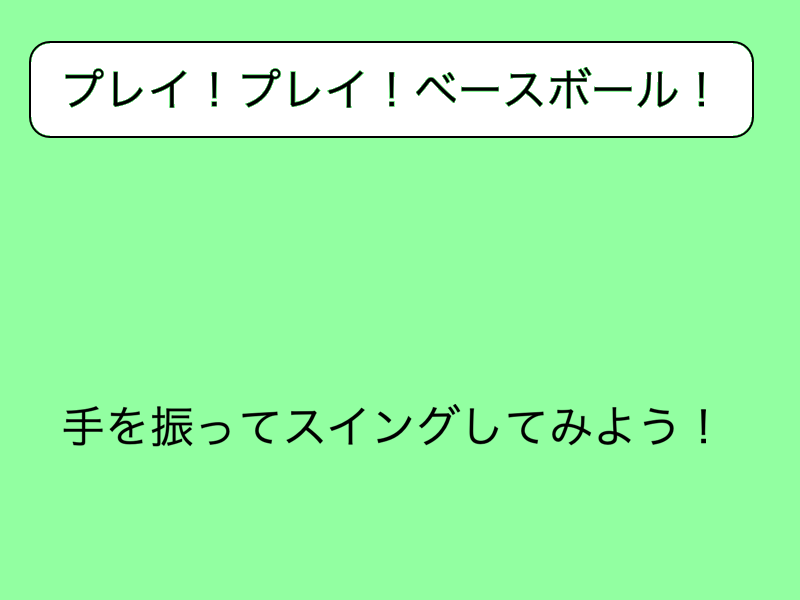
\includegraphics[width=60mm]{title.png}
\caption{タイトル画面}
\label{fig:one}
\end{minipage}
\end{figure}
タイトル画面ではバットを振る動作を確認することができる.そして,zキーを押すことでゲーム画面へ遷移する.
\begin{figure}[htbp]
\begin{minipage}{0.3\hsize}
\centering
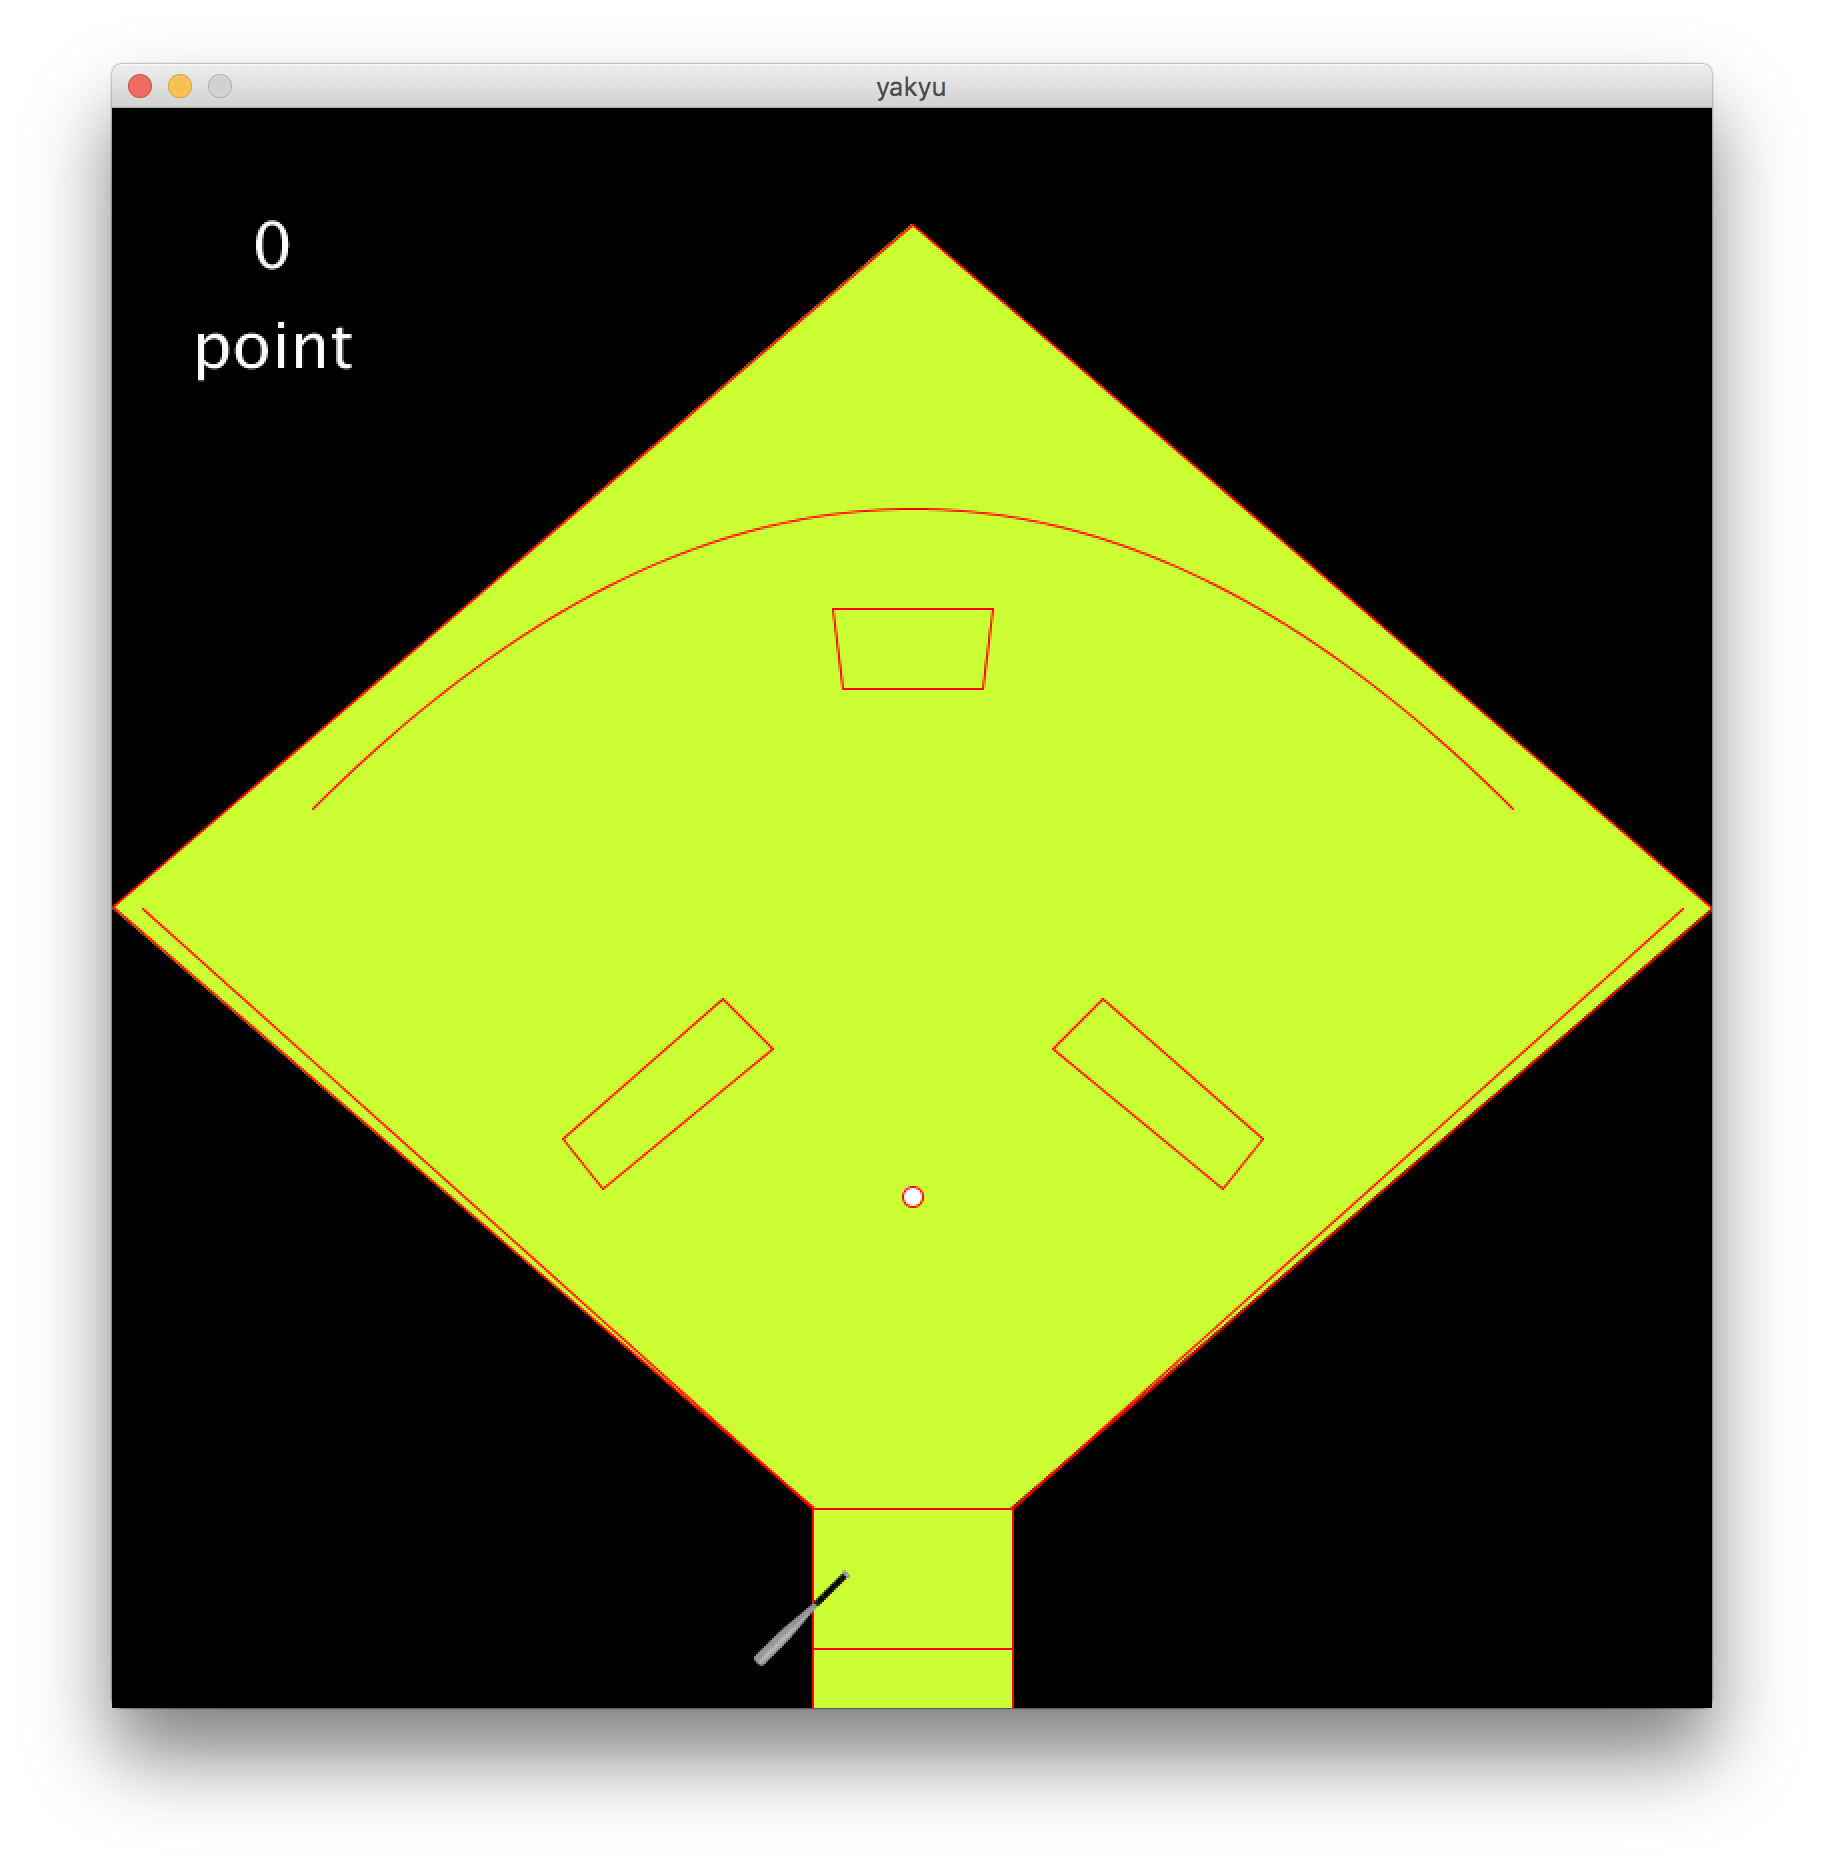
\includegraphics[width=60mm]{yakyu.png}
\caption{ゲーム画面}
\label{fig:two}
\end{minipage}
\end{figure}
ゲーム画面では,中央付近からボールが飛んでくる.それをタイミング良くカメラなどの入力を行うことでボールを打ち返すことができる.
\section{試用結果}
作品の狙いであった簡単にパパッとできるゲームというのを達成することができた.そして,単純なバット振るだけというシステムなため小さい子から野球のルールを知らない人でも楽しむことができる.
\section{発表時に受けたコメント}
カメラを使うには,どうしたら良いかという質問が多かったため,webサイトにリンクを貼っておこうと思います.
\section{今後の課題}
まだクオリティーが高いわけではないので,もう少し投球や,打球や守備などをバリエーションを増やして,いくことでより完成度の高い作品にしていくことが課題となる.
\end{document}
